\chapter{Cadrage géographique}

Le cadrage géographique du projet a constitué une étape méthodologique importante, directement liée à l’hétérogénéité spatiale des données disponibles. Si les données environnementales, météorologiques et astronomiques peuvent être obtenues à des résolutions spatiales fines, les données ouvertes de production photovoltaïque utilisées comme variable cible ne sont, pour leur part, disponibles publiquement qu’à une maille régionale agrégée via la plateforme \textbf{RTE éCO2mix} pour la filière photovoltaïque.

Cette asymétrie imposait de définir une stratégie permettant de rapprocher des variables explicatives locales d’une cible observée à une échelle plus large. Afin d’éviter une représentation trop simplificatrice de la région étudiée, un travail exploratoire de \textbf{clustering géographique} a été mené en amont.

L’approche retenue s’est appuyée sur la répartition géographique du parc de production photovoltaïque régional afin d’identifier plusieurs zones représentatives du territoire. L’objectif était de capturer la diversité des conditions environnementales susceptibles d’influencer la production observée, tout en restant cohérent avec le niveau d’agrégation de la cible. Cette démarche a conduit à la sélection de \textbf{cinq points géographiques représentatifs}, servant de points d’échantillonnage pour la collecte des variables météorologiques, atmosphériques et astronomiques.

Le choix de la région \textbf{Provence-Alpes-Côte d’Azur (PACA)} s’est imposé naturellement comme zone d’étude. La région combine en effet un fort niveau de pénétration photovoltaïque, une ressource solaire importante et une variabilité météorologique suffisamment marquée pour rendre le problème de modélisation particulièrement intéressant. Ce territoire offre ainsi un compromis favorable entre disponibilité des données, cohérence physique et intérêt opérationnel pour l’étude de la variabilité photovoltaïque.


\begin{figure}[htbp]
    \centering
    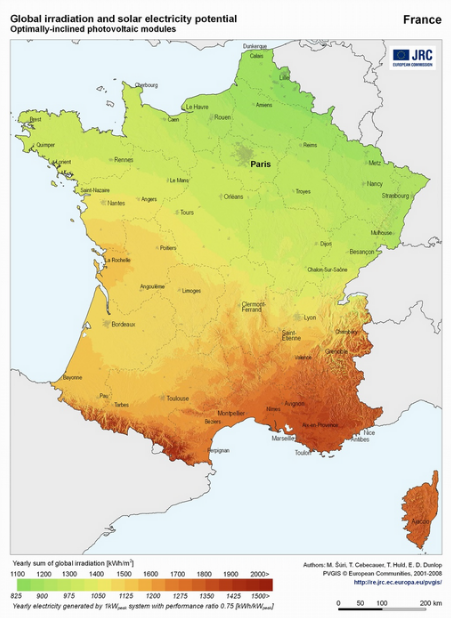
\includegraphics[height=7cm]{img/irradianceFR.png}
    \caption{Irradiance solaire annuelle moyenne en France.}
    \label{fig:irradianceFR}
\end{figure}

Cette carte représente la répartition spatiale de l’irradiance solaire annuelle moyenne sur le territoire français. Elle met en évidence un gradient Nord–Sud marqué, avec des niveaux d’irradiance plus élevés dans le sud du pays, notamment en région Provence-Alpes-Côte d’Azur. Cette distribution contribue à expliquer les disparités régionales observées en matière de production photovoltaïque.
Source : Commission européenne – PVGIS (JRC).
